% =====================================================================
%  Aufgabe 1 – Vorlage für ein Kapitel. Tipp: ein Satz pro Zeile,
%  dann zeigt Git Änderungen satzweise und Konflikte werden seltener.
% =====================================================================
\chapter{Projektthema}
\label{chap:projektthema}

\section{Einleitung}
\label{sec:pt-einleitung}

Im Rahmen dieses Moduls möchten wir die bereits bestehende Webanwendung „tick.it“ weiterentwickeln.
„tick.it“ ist eine Anwendung zur Aufgabenverwaltung, die auf dem Kanban-Prinzip basiert.
Nutzende können Aufgaben erstellen, bearbeiten und löschen sowie diese zwischen verschiedene Spalten verschieben.
Dadurch können Aufgaben übersichtlich organisiert und deren Bearbeitungsstand nachvollzogen werden.\\
Für die Weiterentwicklung haben wir uns für den Consumer-Bereich entschieden.
Unsere primäre Zielgruppe sind Studierende, die ihre Aufgaben, Abgaben und persönlichen Projekte organisieren möchten.
Gerade im Studienalltag müssen häufig mehrere Aufgaben aus unterschiedlichen Modulen gleichzeitig bearbeitet werden.
Dabei kann es schnell unübersichtlich werden, welche Aufgaben noch offen sind, welche bereits begonnen wurden und was schon erledigt ist.
„tick.it“ soll dabei helfen, diese Aufgaben zu strukturieren und den Überblick zu behalten.\\
Als sekundäre Zielgruppe sehen wir Privatpersonen, die beispielsweise ihre Hobbyprojekte oder Aufgaben innerhalb der Familie organisieren möchten.
Auch hier kann eine übersichtliche Aufgabenverwaltung sinnvoll sein, um anstehende Tätigkeiten festzuhalten und den Fortschritt einzelner Aufgaben nachzuvollziehen.\\
Das Projekt entstand ursprünglich im Rahmen des Moduls „Interaktive Systeme“ (WiSe25/26).
An der Entwicklung waren Philipp Wisser und Tara Dethlefsen beteiligt.
Die damalige optionale Aufgabenstellung bestand darin, eine Web-App-Idee umzusetzen und zu präsentieren.\\
Bei „tick.it“ handelt es sich also bereits um eine implementierte Webanwendung und nicht nur um einen grafischen Prototyp.
Neben der grundlegenden Aufgabenverwaltung wurden verschiedene Darstellungsmöglichkeiten wie ein Dark Mode und ein HighContrast-Mode umgesetzt.
Welche Funktionen aktuell vollständig nutzbar sind oder wo es möglicherweise noch technische oder gestalterische Probleme bestehen, muss im weiteren Projektverlauf genauer untersucht werden.\\
Im ursprünglichen Projekt lag der Schwerpunkt auf der technischen Entwicklung und Umsetzung der Anwendung.
Eine Evaluation wurde nicht durchgeführt, daher liegen bislang auch keine konkreten Evaluationsergebnisse vor, aus denen sich Verbesserungsmöglichkeiten ableiten lassen.\\
Im Rahmen der Weiterentwicklung möchten wir uns deshalb genauer damit beschäftigen, wie gut „tick.it“ die Anforderungen unserer Zielgruppe erfüllt und an welchen Stellen die Anwendung noch verbessert werden kann.\\
Unser Ziel ist dabei stärker auf die Bedürfnisse unserer ausgewählten Zielgruppe einzugehen.
Besonders wichtig ist uns, dass die Anwendung einfach zu bedienen ist und eine übersichtliche Organisation verschiedener Aufgaben ermöglicht.\\
Denkbare Verbesserungen wären beispielsweise eine verständlichere Bedienung, eine bessere Übersicht für anstehende Aufgaben oder zusätzliche Funktionen, die besonders für Studierende hilfreich sein könnten.
Welche Änderungen tatsächlich sinnvoll sind und umgesetzt werden sollen, möchten wir im weiteren Projektverlauf genauer untersuchen und festlegen. 

\section{Stand des Projektes}
\label{sec:pt-screenshots}
Im Folgenden zeigen wir den momentanen Stand unseres Projektes auf.\\
Eine voll-implementierte Version der Web-App kann außerdem aufgerufen werden unter \href{https://phlipswis.github.io/tick-it/}{https://phlipswis.github.io/tick-it/}.

\begin{figure}[htbp]
  \centering
  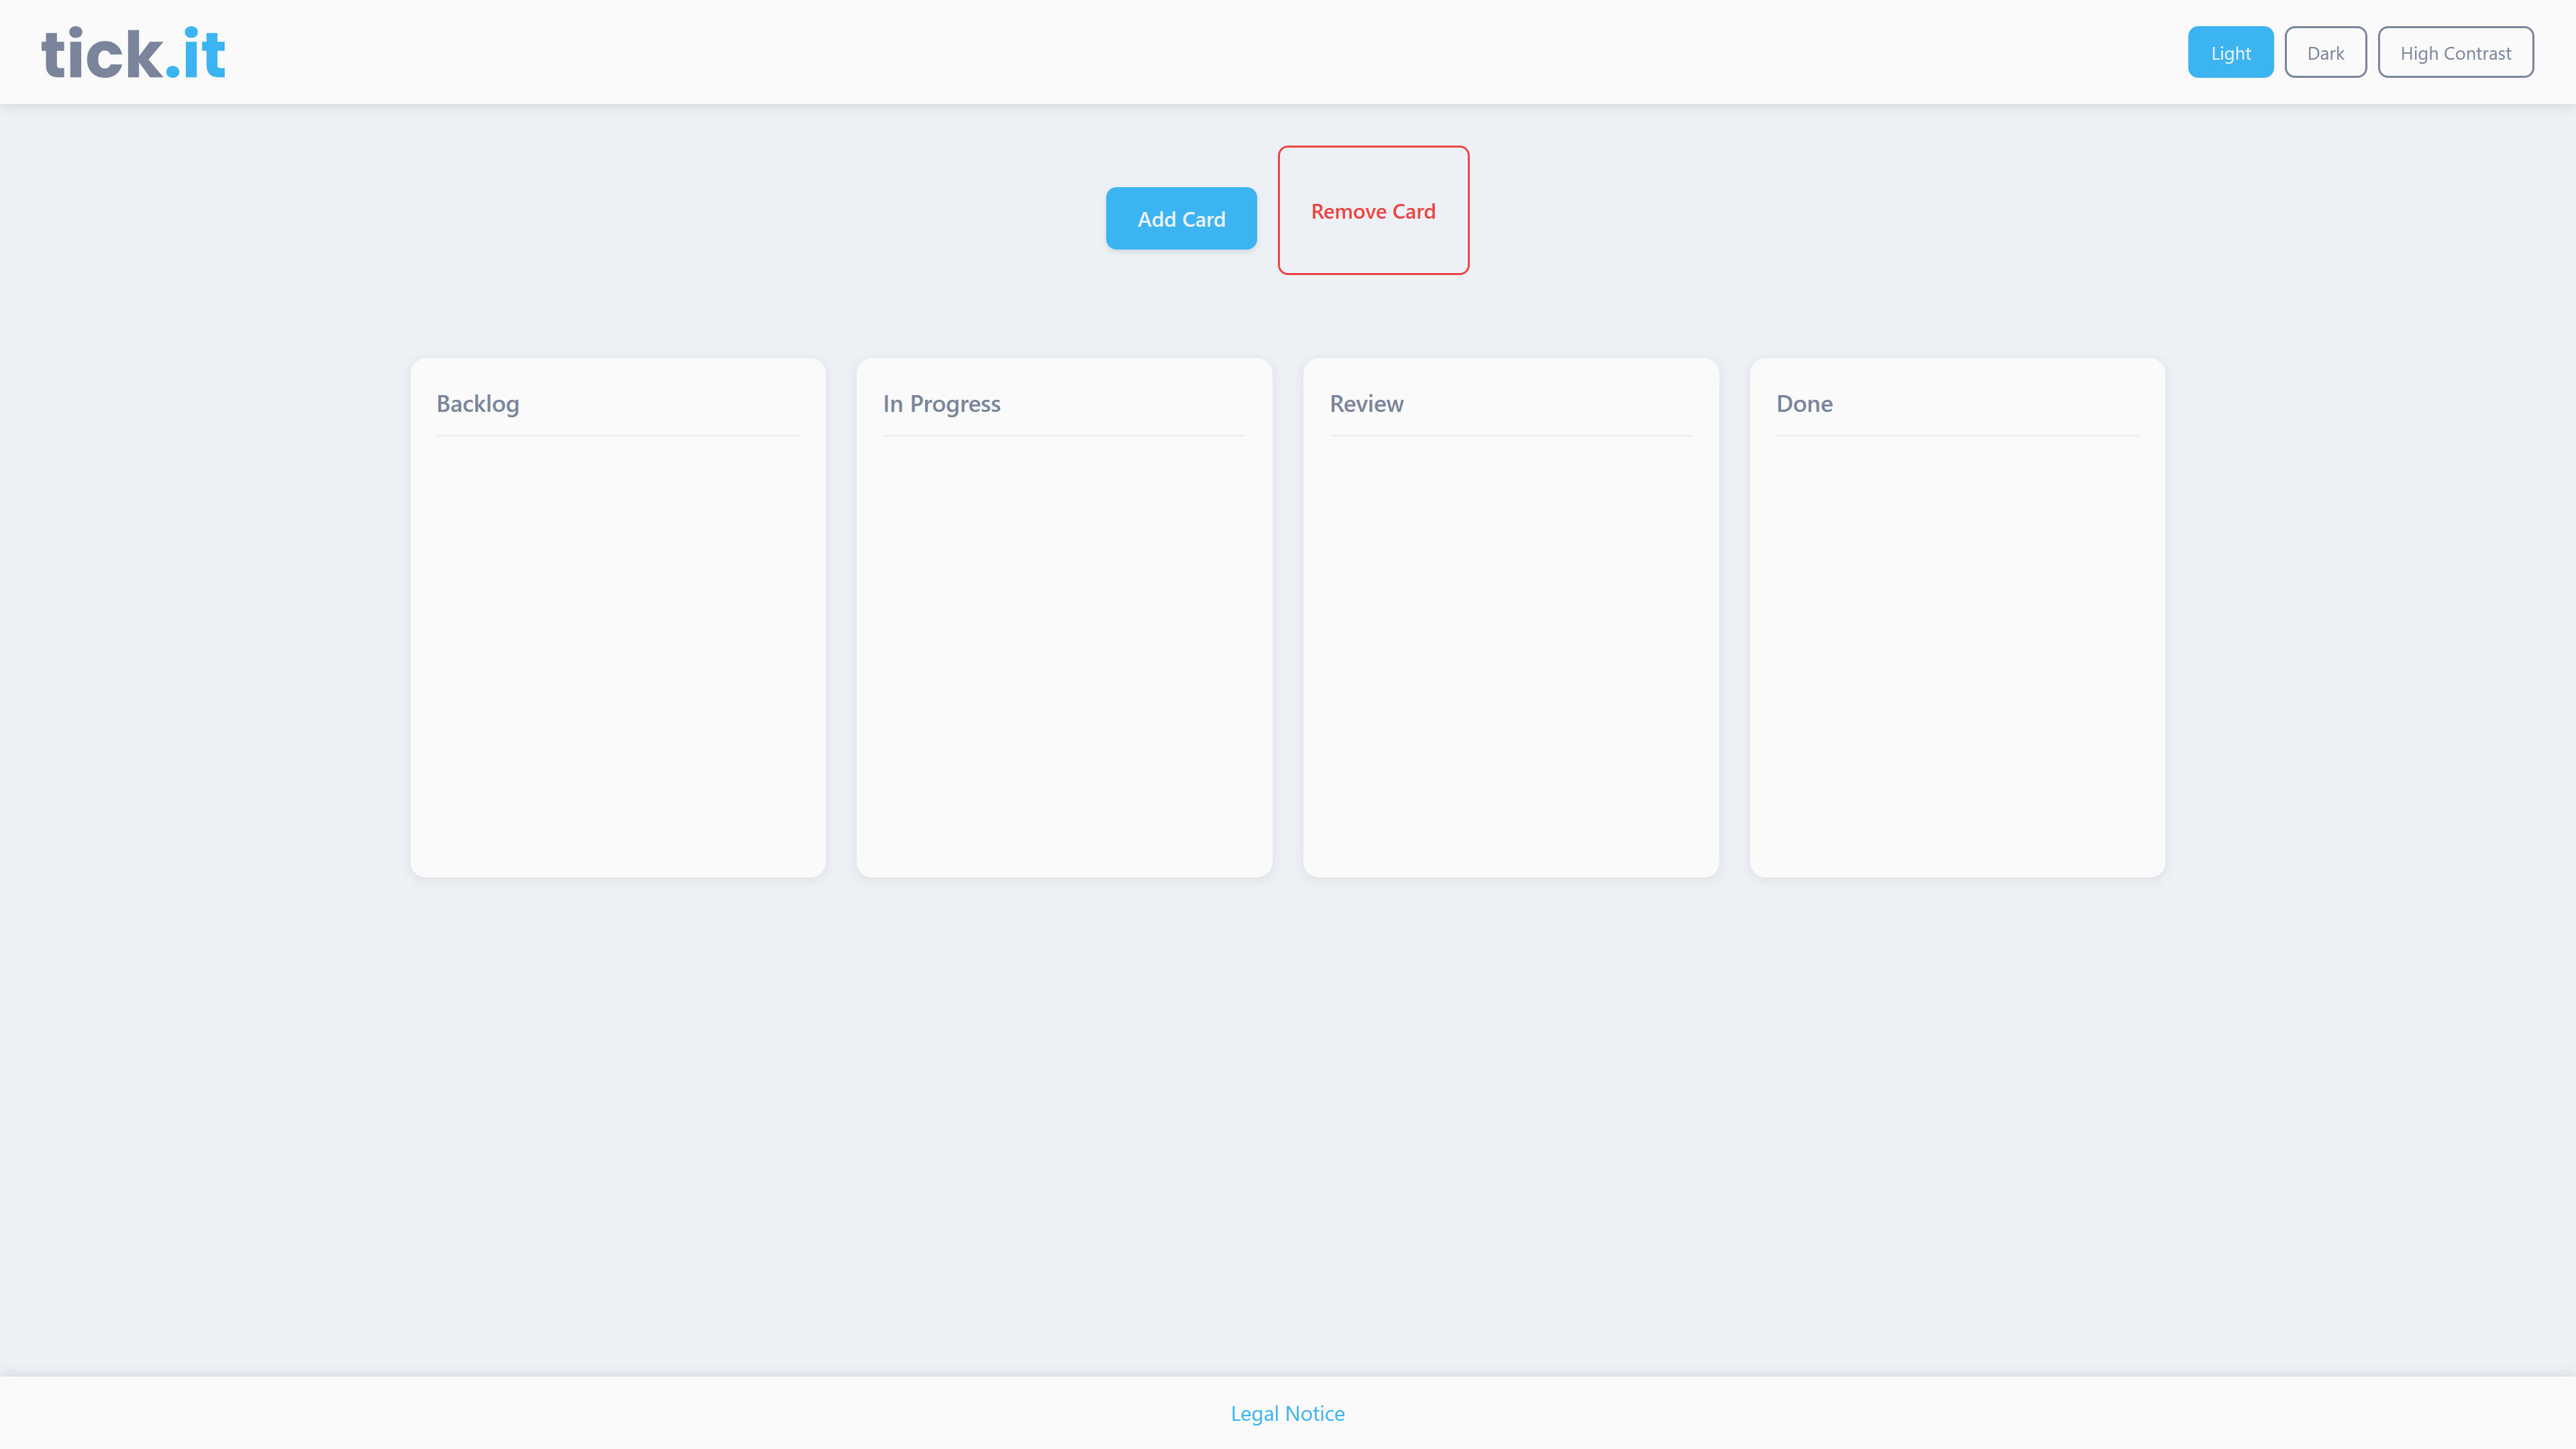
\includegraphics[width=1.0\linewidth]{tick_it_s1.png}
  \caption{tick.it Board \bildquelle{tick-it-page}}
  \label{fig:tick_it_s1}
\end{figure}

\begin{figure}[htbp]
  \centering
  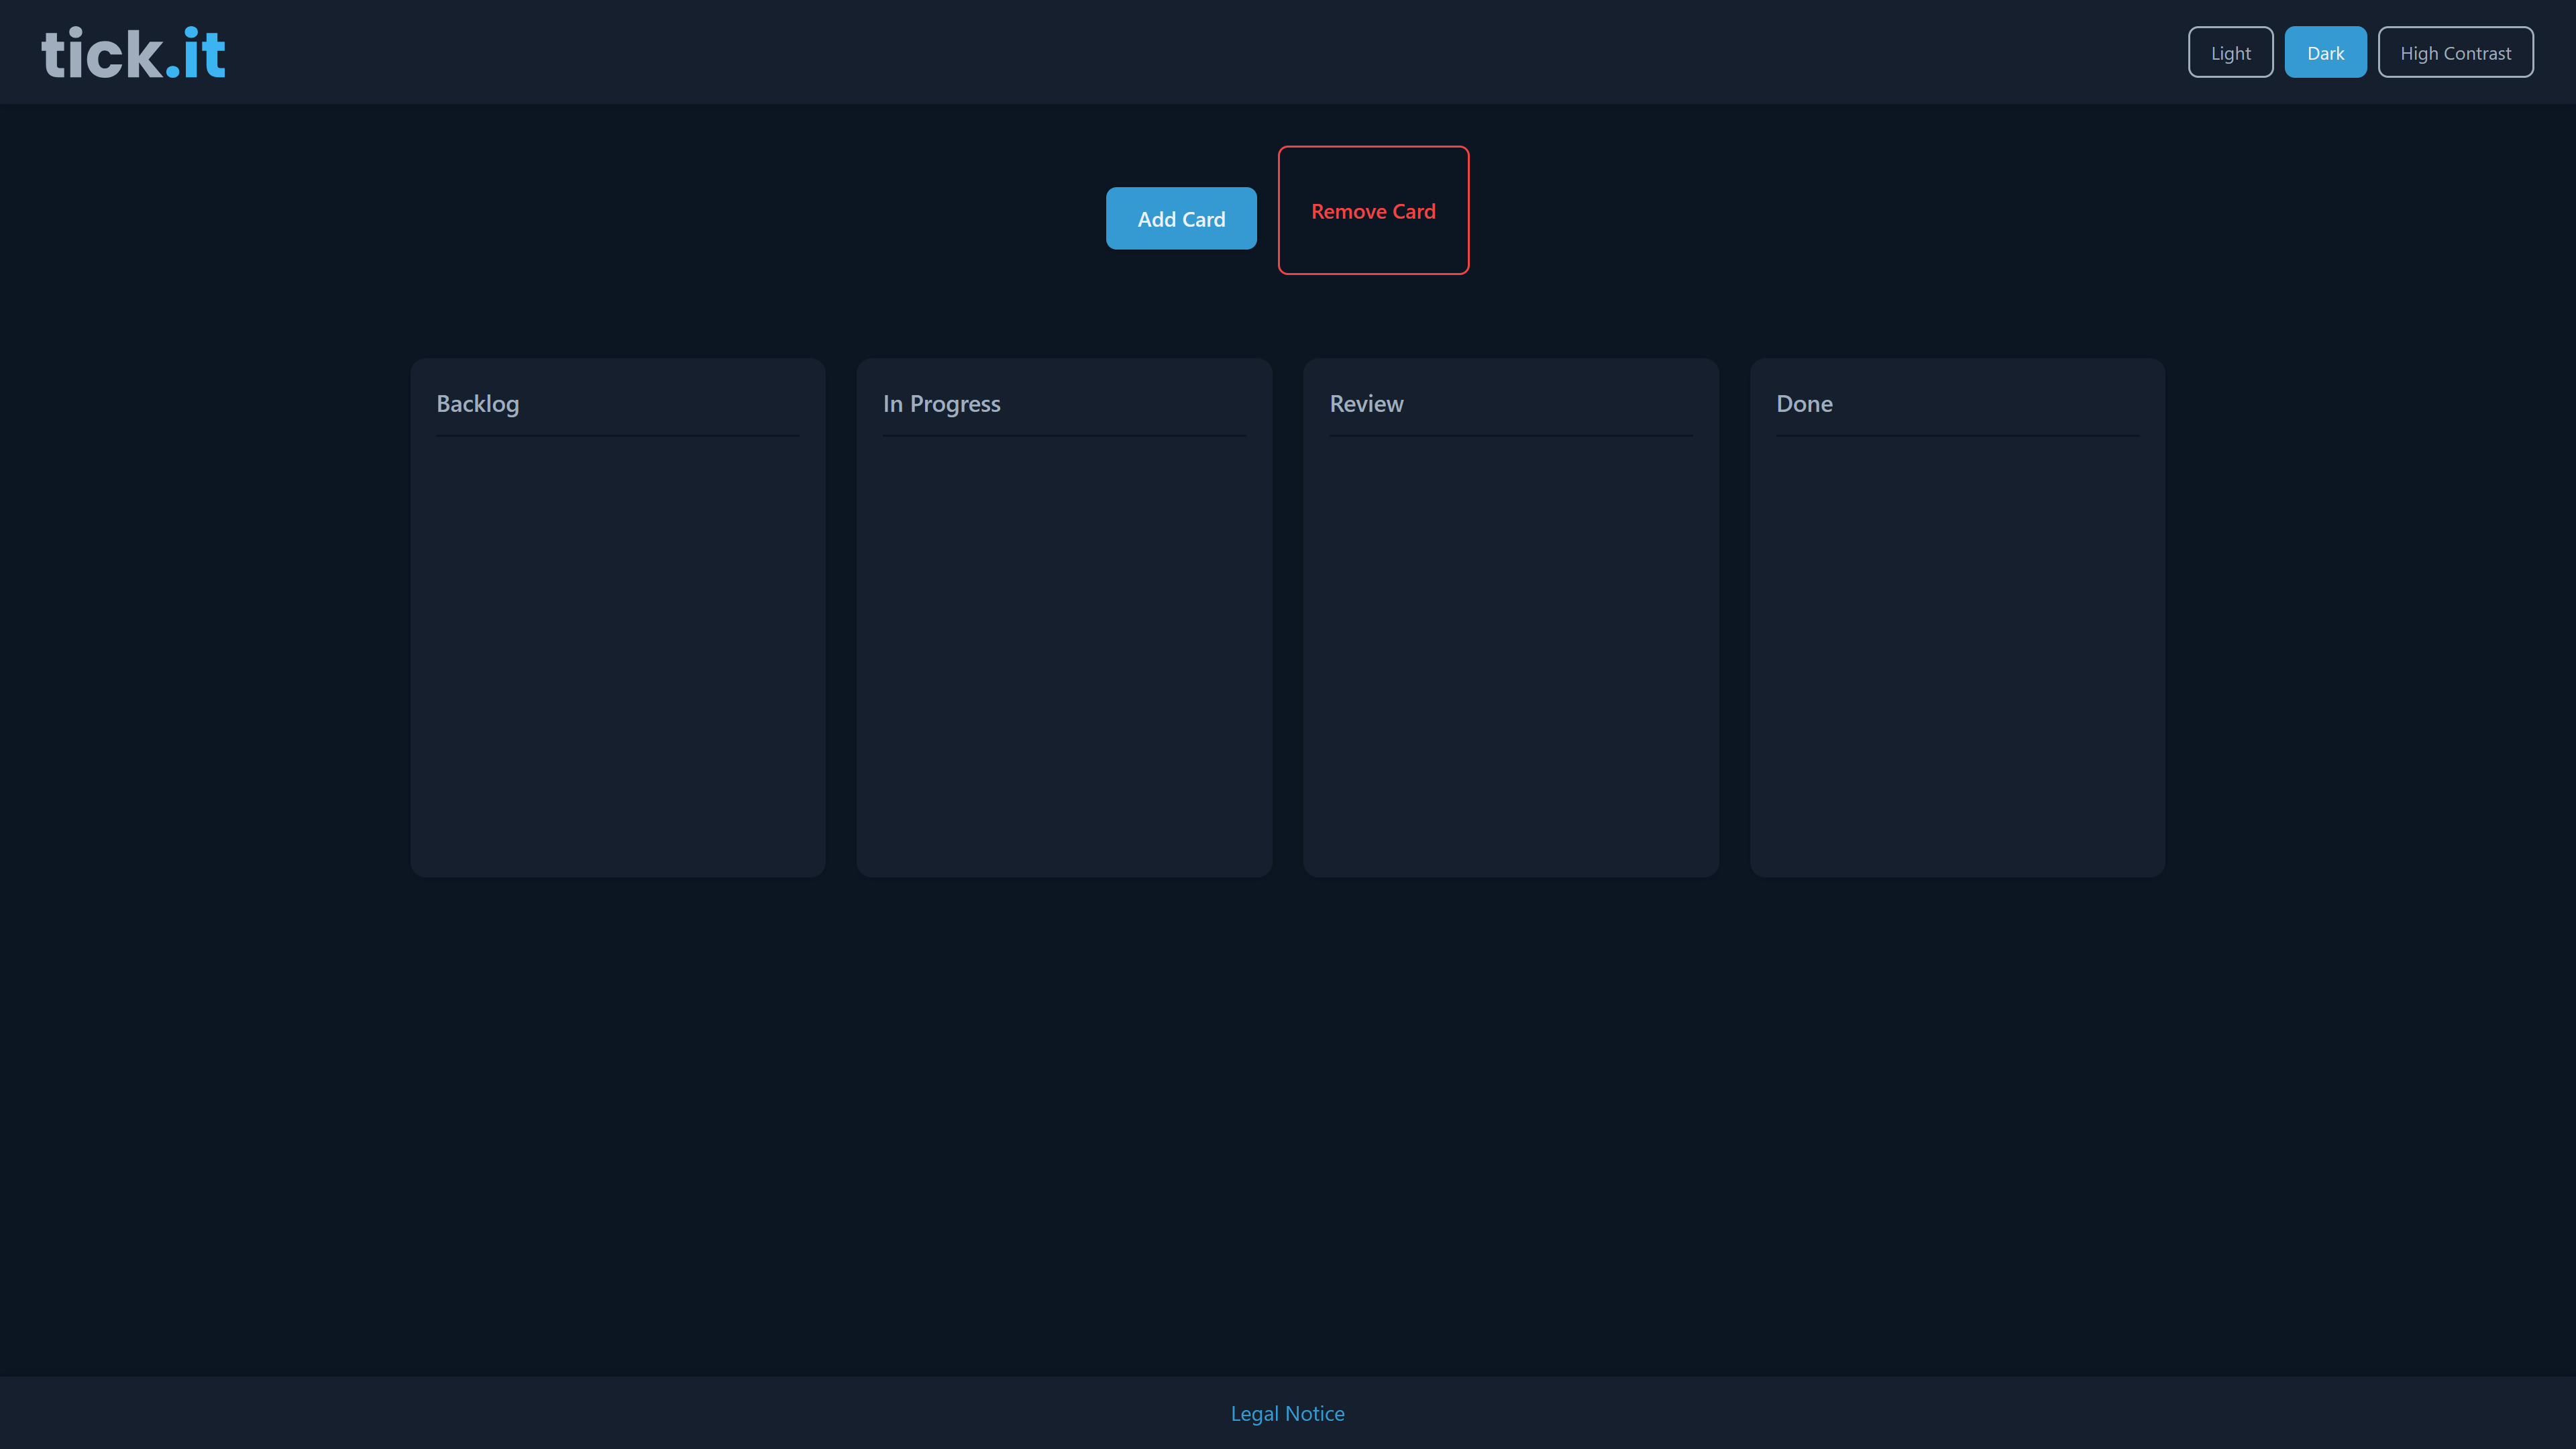
\includegraphics[width=1.0\linewidth]{tick_it_s2.png}
  \caption{tick.it Board Dark Mode \bildquelle{tick-it-page}}
  \label{fig:tick_it_s2}
\end{figure}

\begin{figure}[htbp]
  \centering
  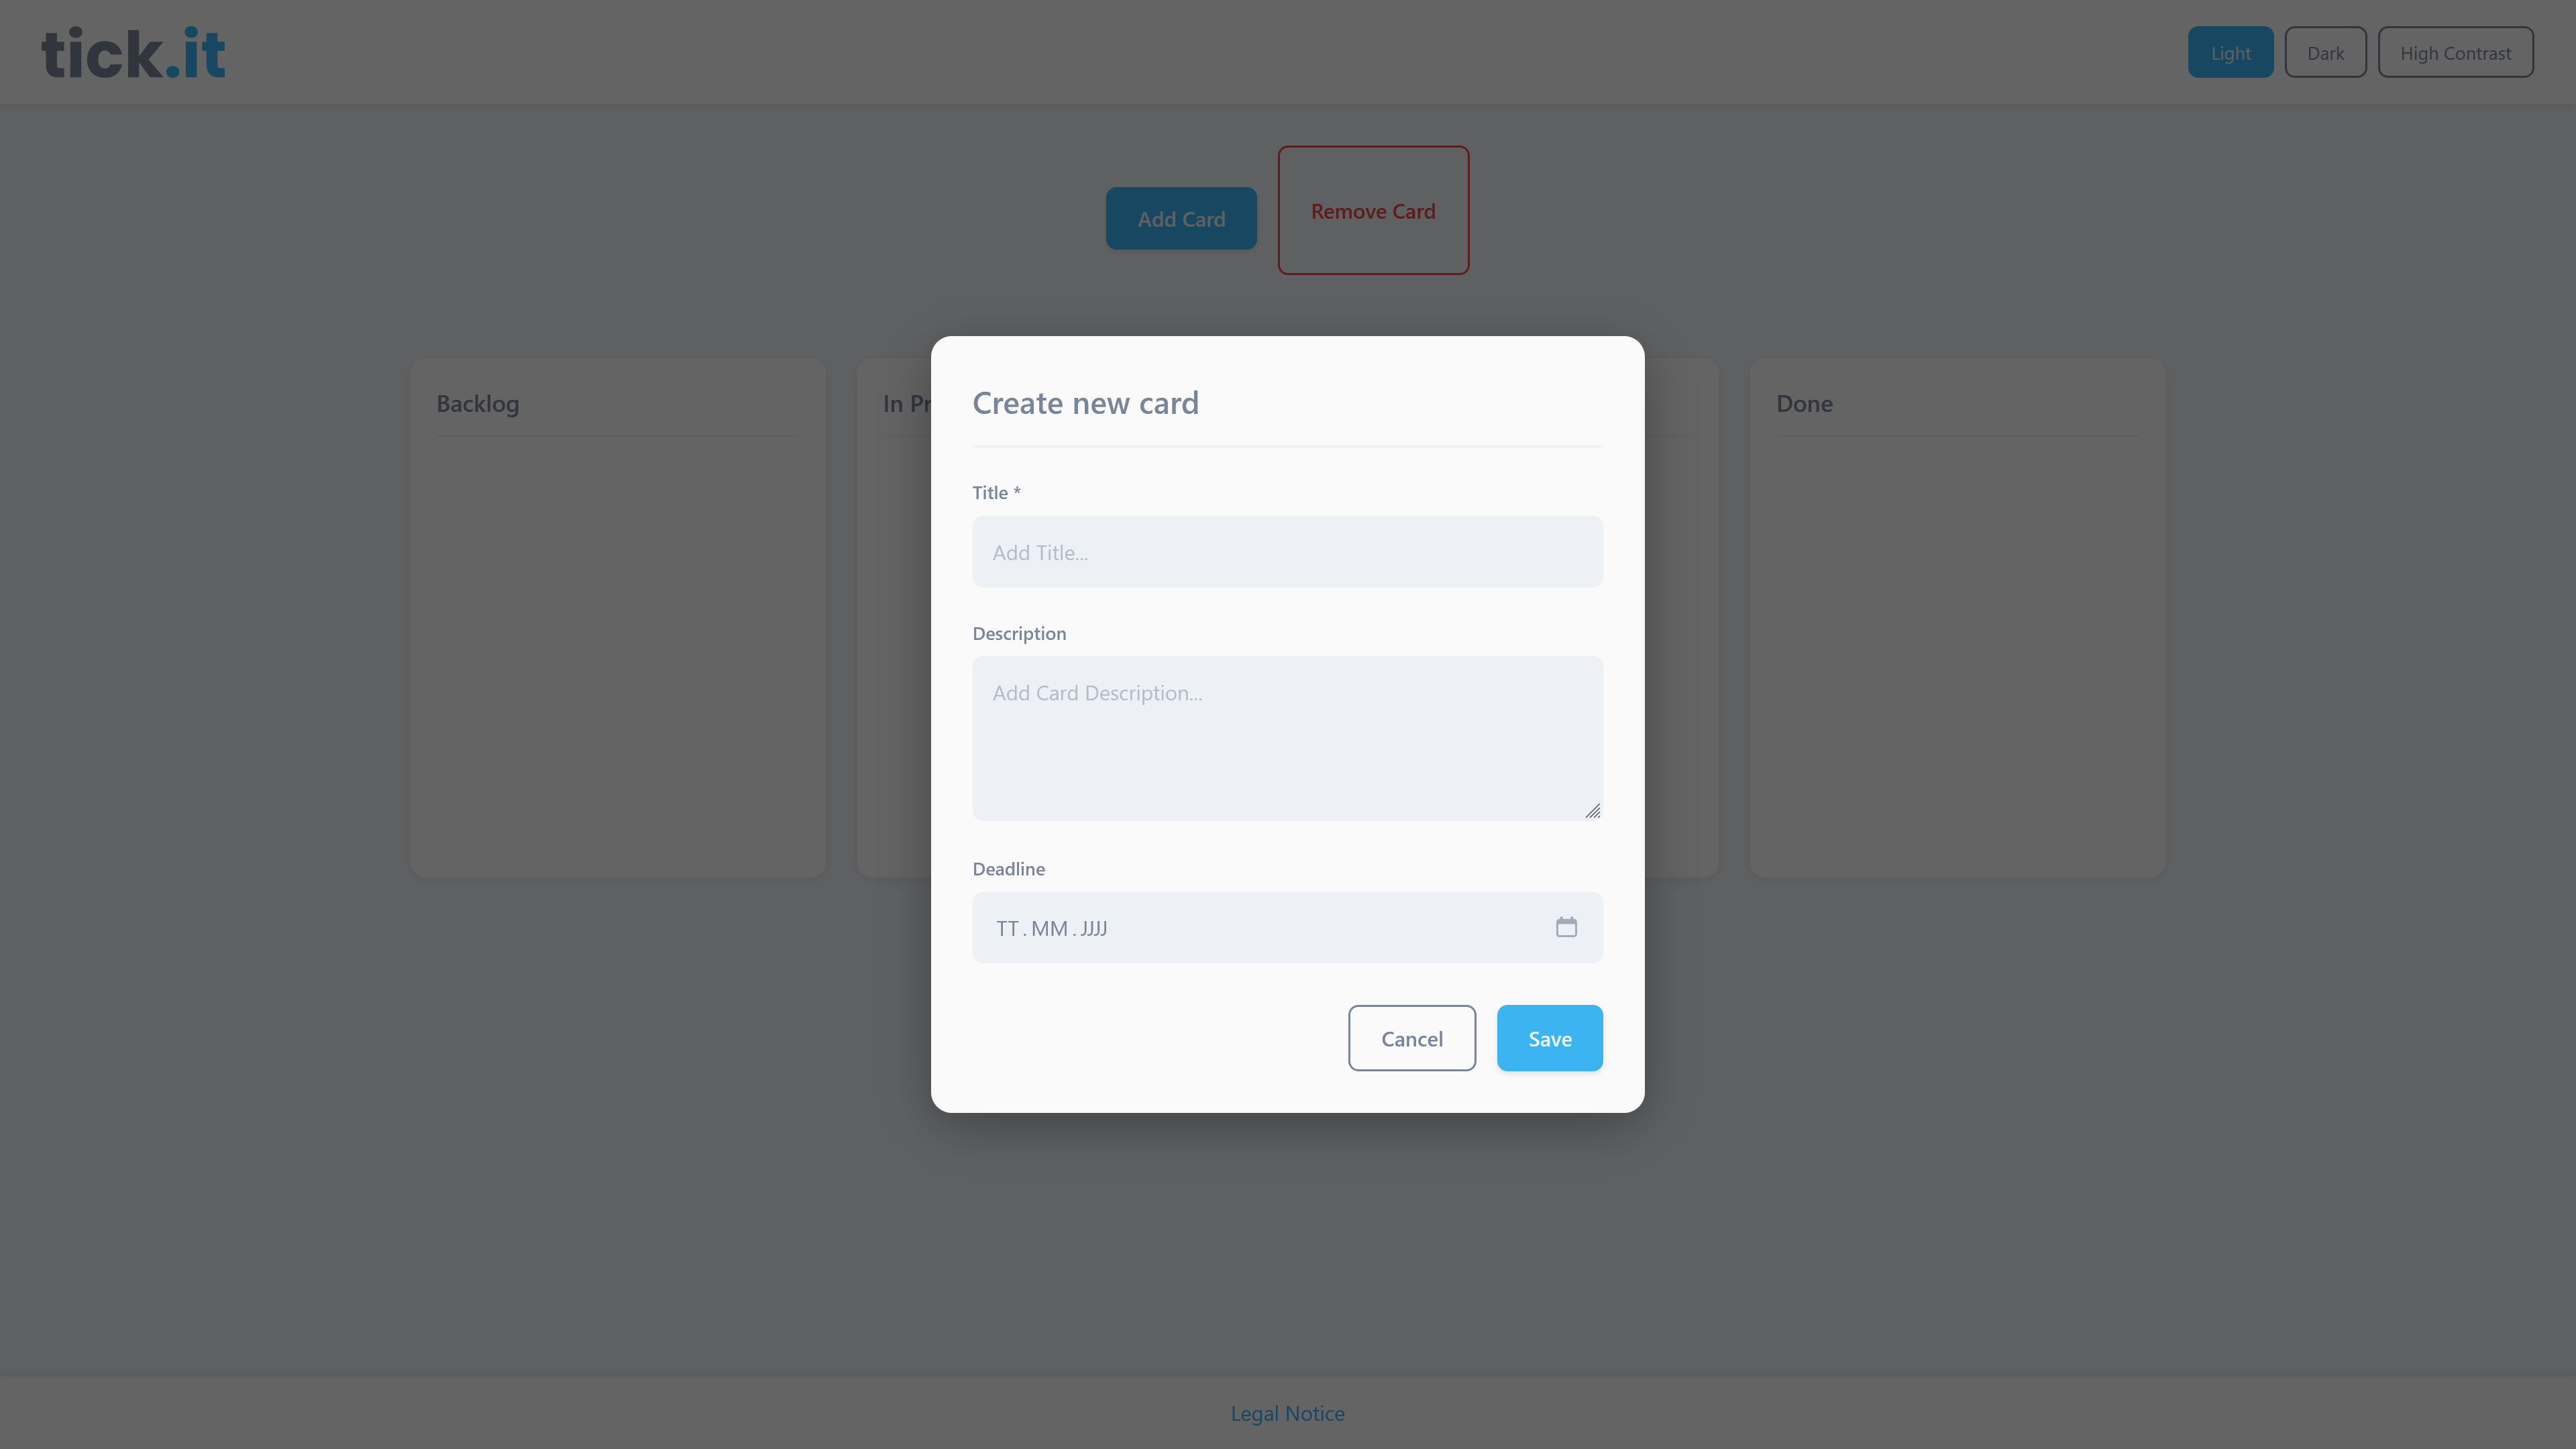
\includegraphics[width=1.0\linewidth]{tick_it_s3.png}
  \caption{tick.it Board Kartenerstellung \bildquelle{tick-it-page}}
  \label{fig:tick_it_s3}
\end{figure}


% ---------------------------------------------------------------------
\begin{beitraege}
  Text \cref{sec:pt-einleitung}                                        & Lara Senger \\
  Anlegen des Projektes & Philipp Wisser \\
  Screenshots \cref{sec:pt-screenshots} & Philipp Wisser \\
  Korrekturlesen & Tara Dethlefsen \\
  \midrule
  KI/Automatisierung: Claude Opus 5.5 zur Erstellung des LaTeX Templates \parencite{claude2026}        & Philipp Wisser \\
\end{beitraege}
